The Fibonacci sequence consists in the sequence: 1,1,2,3,5,8,13,21,34,55,89,144, ... ; where the sequence can be defined as the recurrence relation:

\begin{align*} f_n=f_{n-1}+f_{n-2}\end{align*}

Next, the most significant digit from the first 1000 Fibonacci numbers is obtained, and the frequency of repetition of number 1 as the first digit is calculated, the same can be done with number 2, and so on until number 9. Finally a plot of this frequency distribution against the distribution predicted by Benford's Law is presented.


\begin{figure}[h]
\centering
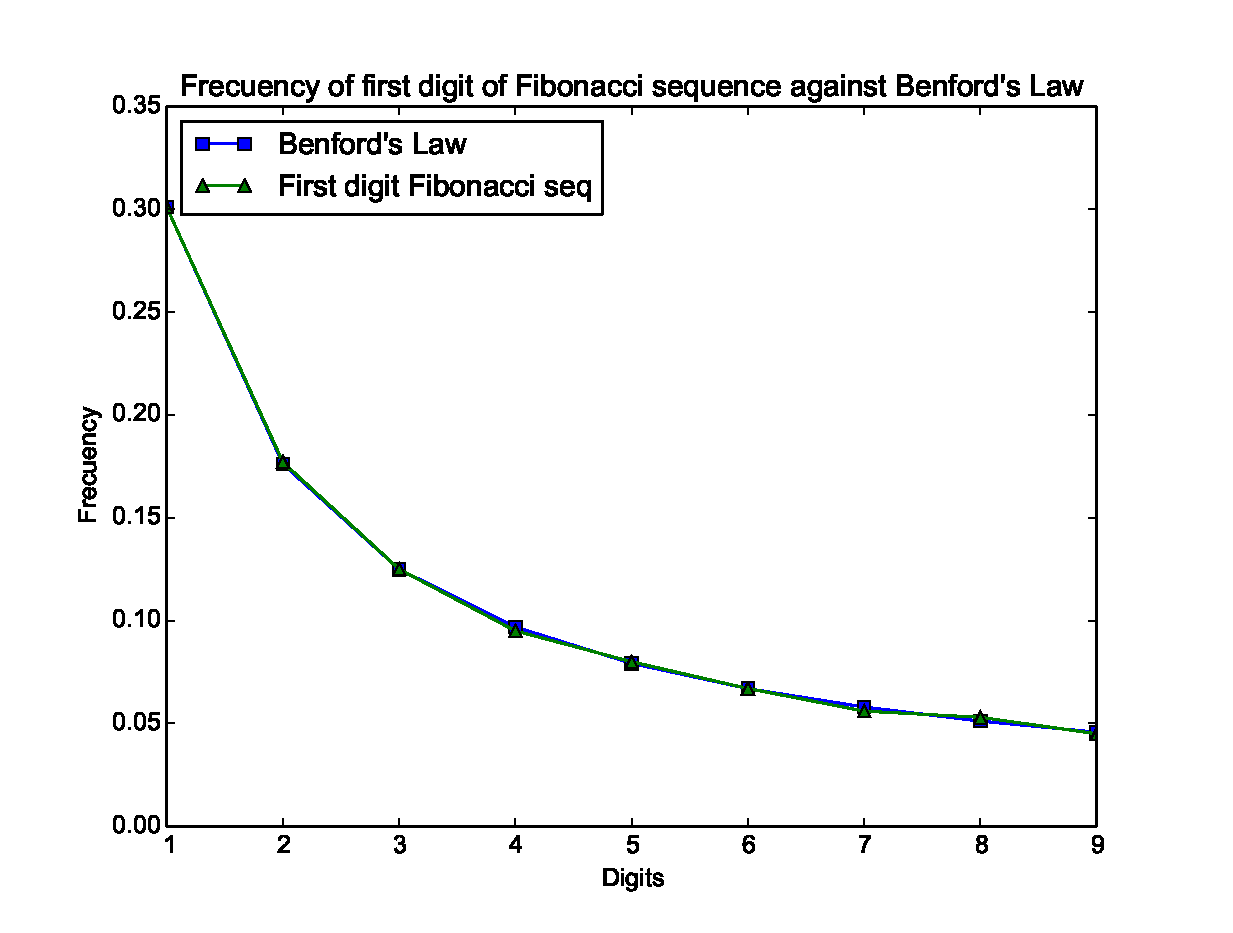
\includegraphics[scale=0.5]{imagenes/2-benford/benford_ex1}
\caption{Fibonacci Sequence against Benford's Law}
\end{figure}
